\documentclass[a4paper,11pt]{article}
\usepackage[utf8]{inputenc}
\usepackage[T1]{fontenc}
\usepackage[swedish]{babel}
\usepackage{amsmath,amssymb,amsfonts}
\usepackage{tikz}
\usepackage{enumitem}
\usepackage{geometry}
\geometry{margin=2.5cm}

\title{Extraövningar: Räta linjens ekvation, linjära funktioner och exponentialfunktioner}
\author{Viktor Arohlén}
\date{\today}

\begin{document}

\maketitle

% Räta linjens ekvation
\section{Räta linjens ekvation}
\begin{enumerate}[label=\textbf{\arabic*.}]
    \item Vad är lutningen för linjen $y = 2x + 1$?
    \item Vad är $y$-värdet när $x = 0$ för linjen $y = -3x + 4$?
    \item Bestäm räta linjens ekvation som går genom punkten $(0,2)$ och har lutningen $k=3$.
    \item Bestäm räta linjens ekvation som går genom punkterna $(1,2)$ och $(3,6)$.
    \item För linjen $y = -x + 5$, bestäm $x$ när $y = 0$.
    \item Bestäm räta linjens ekvation som går genom punkterna $(-2,2)$ och $(4,-10)$.
    \item \textbf{Grafanalys:} Nedan visas grafen till en linje. Svara på frågorna.
    \begin{center}
    \begin{tikzpicture}[scale=0.8]
  % Axlar
  \draw[->] (-1,0) -- (5,0) node[right] {$x$};
  \draw[->] (0,-1) -- (0,5) node[above] {$y$};
  % x-ticks
  \foreach \x in {0,1,2,3,4}
    \draw (\x,0.1) -- (\x,-0.1) node[below] {$\x$};
  % y-ticks
  \foreach \y in {0,1,2,3,4}
    \draw (0.1,\y) -- (-0.1,\y) node[left] {$\y$};
  % Linje
  \draw[thick,blue] (-2,-1) -- (4,5);
\end{tikzpicture}
    \end{center}
    a) Vad är linjens lutning?
    
    b) Vad är linjens ekvation?
    
    c) Var skär linjen $y$-axeln?
\end{enumerate}
\newpage
% Linjära funktioner
\section{Linjära funktioner}
\begin{enumerate}[label=\textbf{\arabic*.}]
    \item För funktionen $f(x) = 2x + 3$, beräkna $f(0)$, $f(2)$ och $f(-1)$.
    \item För funktionen $g(x) = -x + 4$, bestäm $x$ då $g(x) = 1$.
    \item För vilka $x$ gäller $f(x) = g(x)$ om $f(x) = 2x + 3$ och $g(x) = -x + 4$?
    \item \textbf{Grafanalys:} Nedan visas grafen till funktionen $h(x) = -0.5x + 2$.
    \begin{center}
    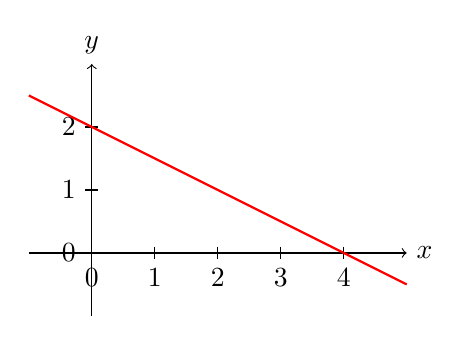
\begin{tikzpicture}[scale=0.8]
  % Axlar
  \draw[->] (-1,0) -- (5,0) node[right] {$x$};
  \draw[->] (0,-1) -- (0,3) node[above] {$y$};
  % x-ticks
  \foreach \x in {0,1,2,3,4}
    \draw (\x,0.1) -- (\x,-0.1) node[below] {$\x$};
  % y-ticks
  \foreach \y in {0,1,2}
    \draw (0.1,\y) -- (-0.1,\y) node[left] {$\y$};
  % Linje
  \draw[thick,red] (-1,2.5) -- (5,-0.5);
\end{tikzpicture}
    \end{center}
    a) Vad är nollstället för $h(x)$?
    
    b) Vad är $h(2)$?
\end{enumerate}
\newpage
% Exponentialfunktioner
\section{Exponentialfunktioner}
\begin{enumerate}[label=\textbf{\arabic*.}]
    \item För funktionen $f(x) = 2^x$, beräkna $f(0)$, $f(1)$, $f(2)$.
    \item För funktionen $g(x) = 3 \cdot 2^x$, bestäm $g(0)$ och $g(2)$.
    \item En exponentialfunktion $h(x) = a \cdot b^x$ har värdet $h(0) = 5$ och $h(1) = 10$. Bestäm $a$ och $b$.
    \item \textbf{Grafanalys:} Nedan visas grafen till funktionen $p(x) = 2^x$.
    \begin{center}
    \begin{tikzpicture}[scale=0.8]
  % Axlar
  \draw[->] (-1,0) -- (4,0) node[right] {$x$};
  \draw[->] (0,-1) -- (0,9) node[above] {$y$};
  % x-ticks
  \foreach \x in {0,1,2,3}
    \draw (\x,0.2) -- (\x,-0.2) node[below] {$\x$};
  % y-ticks
  \foreach \y in {0,2,4,6,8}
    \draw (0.2,\y) -- (-0.2,\y) node[left] {$\y$};
  % Graf
  \draw[thick,green!70!black,domain=-1:3,samples=40] plot (\x,{2^\x});
\end{tikzpicture}
    \end{center}
    a) Vilket värde har $p(2)$?
    
    b) Vad är $p(0)$?
    
    c) Hur förändras $p(x)$ när $x$ ökar med 1?
\end{enumerate}
\newpage
% Problemlösning med funktioner
\section{Problemlösning med funktioner}
\begin{enumerate}[label=\textbf{\arabic*.}]
    \item En biobiljett kostar 90 kr. Skriv en funktion $C(x)$ som beskriver totalkostnaden för $x$ biljetter. Vad kostar 5 biljetter?
    \item En cykelbutik hyr ut cyklar för 80 kr per dag plus en fast avgift på 50 kr. Skriv en funktion $H(x)$ för hyran av $x$ dagar. Vad kostar det att hyra i 3 dagar?
    \item En bakteriekultur fördubblas varje timme och startar med 10 bakterier. Skriv en funktion $N(t)$ som beskriver antalet bakterier efter $t$ timmar. Hur många bakterier finns efter 4 timmar?
    \item Nedan visas grafen till en funktion $f(x)$ av tredje graden.
    \begin{center}
    \begin{tikzpicture}[scale=0.8]
      % Axlar
      \draw[->] (-3,0) -- (4,0) node[right] {$x$};
      \draw[->] (0,-3) -- (0,5) node[above] {$y$};
      % x-ticks
      \foreach \x in {-2,-1,1,2,3}
        \draw (\x,0.15) -- (\x,-0.15) node[below] {$\x$};
      % y-ticks
      \foreach \y in {-2,2,4}
        \draw (0.15,\y) -- (-0.15,\y) node[left] {$\y$};
      % Graf: t.ex. f(x) = (x+2)(x-1)(x-3)/2 + 1
      \draw[thick,blue,domain=-2.2:3.2,samples=100,smooth] plot (\x,{((\x+2)*(\x-1)*(\x-3))/2 + 1});
    \end{tikzpicture}
    \end{center}
    a) Vad är $f(0)$?
    
    b) För vilka $x$ gäller $f(x) = 0$?

    \item Nedan visas grafen till en annan funktion $g(x)$ av tredje graden.
    \begin{center}
    \begin{tikzpicture}[scale=0.8]
      % Axlar
      \draw[->] (-4,0) -- (4,0) node[right] {$x$};
      \draw[->] (0,-4) -- (0,4) node[above] {$y$};
      % x-ticks
      \foreach \x in {-3,-2,-1,1,2,3}
        \draw (\x,0.15) -- (\x,-0.15) node[below] {$\x$};
      % y-ticks
      \foreach \y in {-2,2}
        \draw (0.15,\y) -- (-0.15,\y) node[left] {$\y$};
      % Graf: t.ex. g(x) = (x+3)(x)(x-2)/3
      \draw[thick,red,domain=-3.3:2.3,samples=100,smooth] plot (\x,{((\x+3)*(\x)*(\x-2))/3});
    \end{tikzpicture}
    \end{center}
    a) Vad är $g(0)$?
    
    b) För vilka $x$ gäller $g(x) = 0$?

\end{enumerate}

\end{document}
